\newpage
\section{Destination Tickets}

\subsection{Winning}
An obvious strategy in \textit{Ticket to Ride} is to collect
Destination Tickets and focus on claiming routes to connect them.
We investigate the effect of collecting Destination Tickets
on winning the game.
We simulate 10,000 two-player and 10,000 four-player games.
For each Destination Ticket, we calculate the proportion of 
games that the player holding the Destination Ticket won.
Our results appear in \cref{fig:tickets}.
(For example, players in two-player games with Montreal 
to Vancouver won almost $60\%$ of their games.)

\begin{figure}[h]
\centering
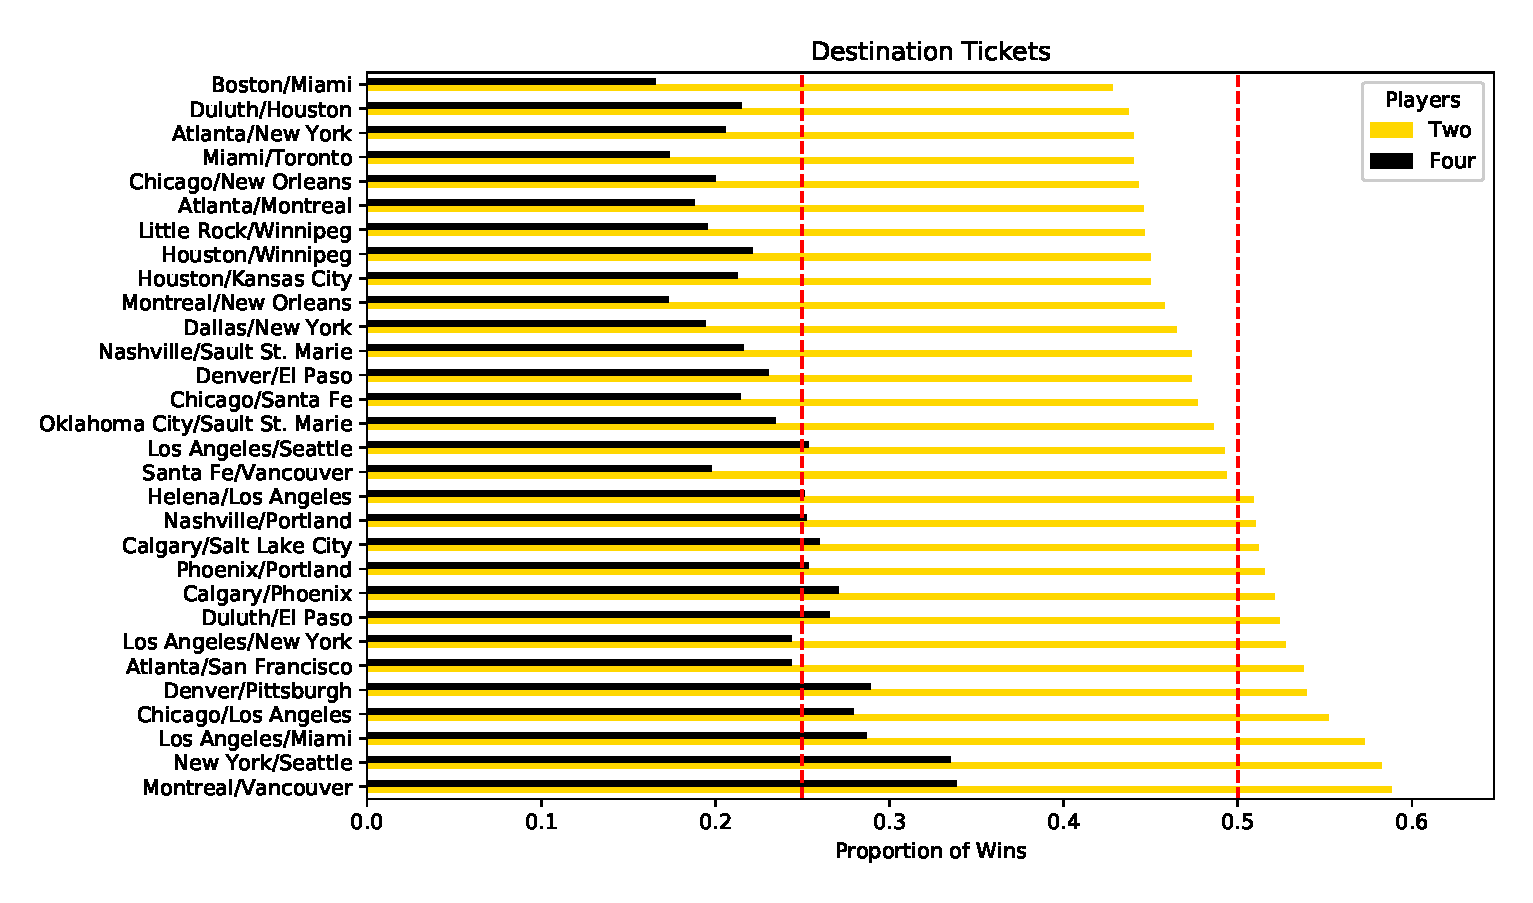
\includegraphics[scale=.6]{figures/destination_tickets}
\caption{For each Destination Ticket,
the proportion of two-player and four-player games that 
the player with the Destination Ticket won.
The vertical red lines at $1/4$ and $1/2$ represent
the expected proportion of games players would win
if Destination Tickets had no effect.}
\label{fig:tickets}
\end{figure}

The vertical red lines at .25 and .5 indicate
the expected proportion of wins if Destination Tickets
had no effect on winning: players in two-player games
would win half the time and players in four-player games
would win a quarter of the time.

In two-player games, there are 13 Destination Tickets 
that win more than the expected $50\%$ of games.
(We say that a Destination Ticket "wins" in the sense
that the players who possesses it wins the game they
are playing.)
In four-player games, there are only eight Destination Tickets
that clearly win more than the expected $25\%$ of games plus
another four on the borderline.
That is, out of the 30 Destination Tickets, roughly a third
in both two- and four-player games win more than expected.
The implication is that a randomly chosen Destination 
Ticket is not advantageous.
However, a subset of Destination Tickets--approximately the same
set for both two- and four-player games--wins more often than expected.
The ones that win the most are Montreal to Vancouver,
New York to Seattle, and Chicago to Los Angeles.

An inspection of \cref{fig:board} shows that the paths between 
these three Destination Tickets include the longest routes
on the board.
However, to gain a better understanding of what makes some
Destination Tickets more advantageous than others,
we investigate their characteristics
that most closely correlate with winning.
We begin in the next subsection by developing a measure
of the difficulty of connecting one city to another.

\subsection{Effective Resistance}
The \textit{Ticket to Ride} board can be mathematically
interpreted as a graph where cities represent
nodes and routes represent edges.
One of the most powerful and natural measures of connectivity
between two nodes on a graph is effective resistance
\cite{ellens2011effective}.
Imagine that the \textit{Ticket to Ride} board were
a large electrical circuit with a unit current
entering at city $a$ and leaving at city $b$.
Effective resistance indicates
how much work a current needs to exert
to get from $a$ to $b$.
In general, the number of paths and length of routes 
determine the effective resistance:
two cities with fewer paths and longer routes
have a higher effective resistance between them
than two cities with many paths and shorter routes.
We calculate the effective resistance for each 
Destination Ticket in order to gain insight
into what makes some more advantageous than others.

On a small graph, effective resistance can be calculated
by repeatedly applying the following rules:
Consider two edges with resistances $r_1$ and $r_0$.
If the two edges are in series (edge 1 connects node $i$ to $j$
and edge 2 connects node $j$ to $k$), then the resistance between
$i$ and $k$ is $r_1 + r_2$.
If the two edges are in parallel (both edge 1 and edge 2 connect
node $i$ to $j$), then the resistance between $i$ and $j$
is $(1/r_1 + 1/r_2)^{-1}$.

On a large graph like the \textit{Ticket to Ride} board, 
we need a more robust strategy.
We use two separate algorithms to find the effective resistance
of Destination Tickets
\cite{ellens2011effective, wu2004theory}.
Both algorithms calculate the effective resistance by finding 
the eigenvalues of the Laplacian matrix for a given graph.
(The Laplacian is the degree matrix $D$ minus the adjacency
matrix $A$ where $D_{i,i}$ is the weighted degree of node $i$
and $A_{i,j}$ is the resistance of the edges between nodes
$i$ and $j$.)

We let the weight between two cities be the length
of the route connecting them.
In the case that there are two routes between cities,
we let the weight be $(1/r + 1/r)^{-1}=r/2$ where
$r$ is the length of each route.
(There are at most two routes between any two cities
on the \textit{Ticket to Ride} board \cref{fig:board}.)

In the next subsection, we calculate the effective
resistance of all Destination Tickets as a tool
to find what most closely correlates with winning.

\begin{figure}[h]
    \centering
    \includegraphics[scale=.6]{figures/resistance_aggregate}
    \caption{Destination Tickets plotted by their effective
    resistance and minimum path length and colored
    by overall proportion of wins.
    The line of best fit gives an approximation of the
    Destination Tickets that have a higher reward per difficulty
    (above the line).
    Note: the $9^{th}$ Destination Ticket 
    is obscured by the $11^{th}$.}
    \label{fig:resistance}
\end{figure}

\subsection{Winning \& Effective Resistance}

In \cref{fig:resistance},
Destination Tickets are plotted by 
the effective resistance 
and minimum path length of the pair of cities they specify.
Recall that the reward for connecting a Destination Ticket
is the length of the shortest path between its two cities.
Since effective resistance measures the difficulty of
connecting the two cities, the line of best fit in \cref{fig:resistance}
indicates reward per difficulty.
The Destination Tickets above the line of best fit are
a "good" deal relative to the rest of the Destination Tickets,
whereas those below the line of best fit are a "bad" deal.

The proportion of wins (also denoted overall wins
in \cref{fig:correlation_table} and \cref{fig:correlation_figures})
is the difference from the expected proportion of wins
across two- and four-player games.
For example, a Destination Ticket with a value of .05 indicates
that players with that destination Ticket 
win on average $30\%$ of four-player games
(rather than the expected $25\%$) and $55\%$ of 
two-player games (rather than the expected $50\%$).

We use the proportion of wins as a proxy for the desirability
of Destination Tickets and attempt to interpret what variables
increase player wins from \cref{fig:resistance}.
It appears that Destination Tickets with longer minimum paths win
more as well as Destination Tickets with 
a smaller effective resistance.
But the correlation between either variable and the proportion
of wins is not clear-cut.

\cref{fig:correlation_table} shows the Pearson 
correlation coefficient
between wins and various (possibly) related variables.
The path length and resistance are the y- and x-axes of 
\cref{fig:resistance}.
The residual is the difference between the predicted
path length (line of best fit) and the actual path length
in \cref{fig:resistance}.
% more intuitive and formal definition of residual
The results indicate that path length is well correlated with wins,
resistance is not correlated with wins, and residual is very
well correlated with wins.
\cref{fig:correlation_figures} shows the data points and
their relationship to wins summarized in
in the last column of \cref{fig:correlation_table}.

\begin{figure}[h]
    \centering
    \includegraphics[scale=.12]{figures/pearsons_table.png}
    \caption{The Pearson correlation statistic between
    the win proportion of Destination Tickets
    and measures of difficulty.
    A single asterisk (in light green) indicates a p-value
    below 1E-2. Double asterisks (in green) indicate a
    p-value below 1E-4. Triple asterisks (in dark green)
    indicate a p-value below 1E-6.}
    \label{fig:correlation_table}
\end{figure}

\begin{figure}[H]
    \centering
    \begin{subfigure}[t]{0.36\textwidth}
        \centering
        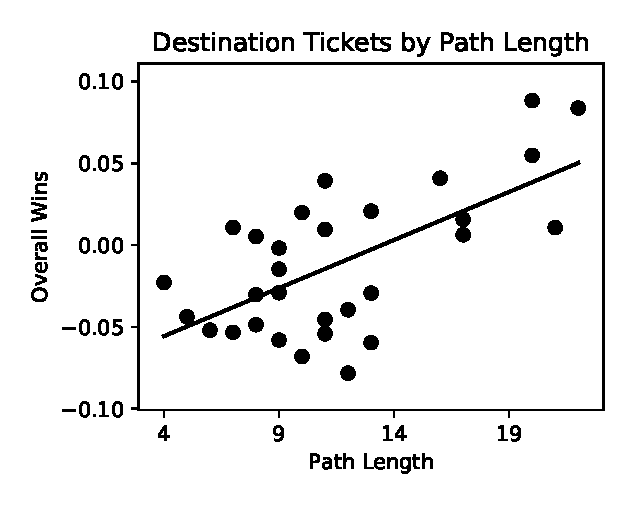
\includegraphics[height=1.7in]{figures/correlation0}
    \end{subfigure}%
    ~ 
    \begin{subfigure}[t]{0.36\textwidth}
        \centering
        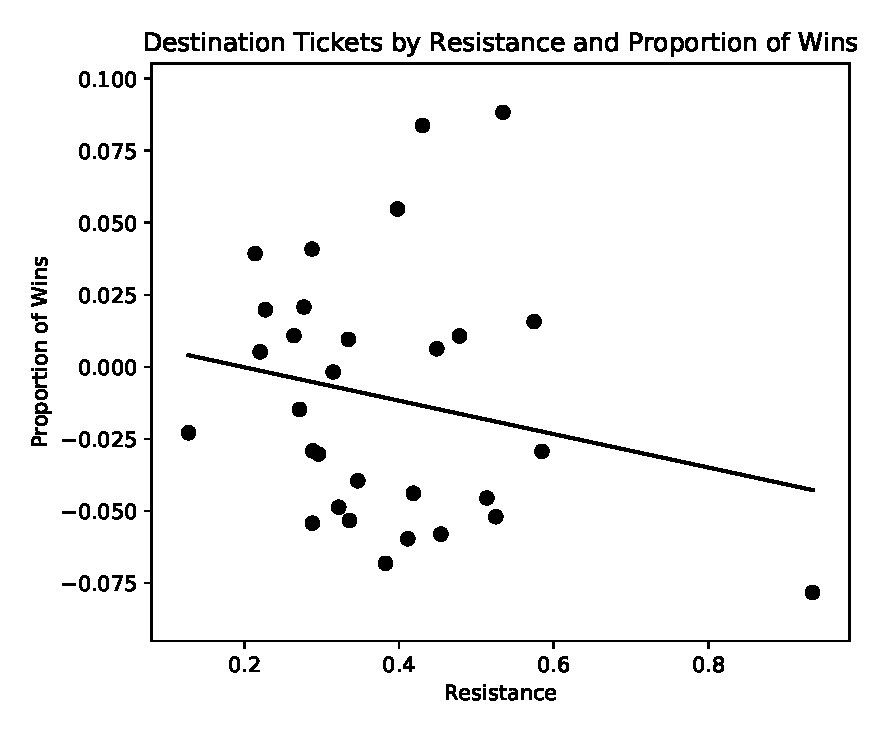
\includegraphics[height=1.7in]{figures/correlation1}
    \end{subfigure}%
    ~ 
    \begin{subfigure}[t]{0.36\textwidth}
        \centering
        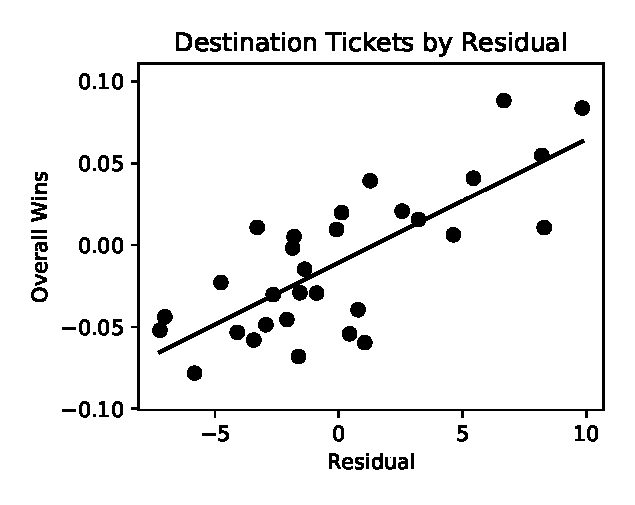
\includegraphics[height=1.7in]{figures/correlation2}
    \end{subfigure}%
    \caption{Destination Tickets by the
    difference between the expected proportion of wins
    and (possibly) related variables.
    The last column of \cref{fig:correlation_figures}
    indicates how closely the lines of best fit
    model Destination Tickets.}
    \label{fig:correlation_figures}
\end{figure}

While path length is a good predictor 
of which Destination Tickets win, 
the residual from the model built from effective resistance
is even better (\cref{fig:correlation_table} and
\cref{fig:correlation_figures}).
\cref{fig:rankings} shows the change in rankings
between path length and residual.

Even though it is easier to compare path length when choosing
between Destination Tickets in real time,
learning the most advantageous Destination Tickets may be worthwhile:
as a general rule, Destination Tickets with a minimum path
length above 15 or those with small effective resistance
(many short paths) outperform their counterparts.

Referring to \cref{fig:resistance}, 
we provide several explanations for why certain
Destination Tickets win more than expected.
The Destination Tickets with length greater than 15 
enjoy high rewards and middle-of-the-pack 
resistances.
In addition, they benefit from the advantages of longer 
routes discussed in \cref{sec:overvalued}.
The remaining Destination Tickets--below or slightly 
above the line of best fit--seem to be more affected
by resistance: the higher the resistance, the
lower the proportion of wins.
Perhaps because the resistance between these pairs of cities
is roughly comparable, Destination Tickets that 
can be connected more easily help players more.

\begin{figure}[H]
    \centering
    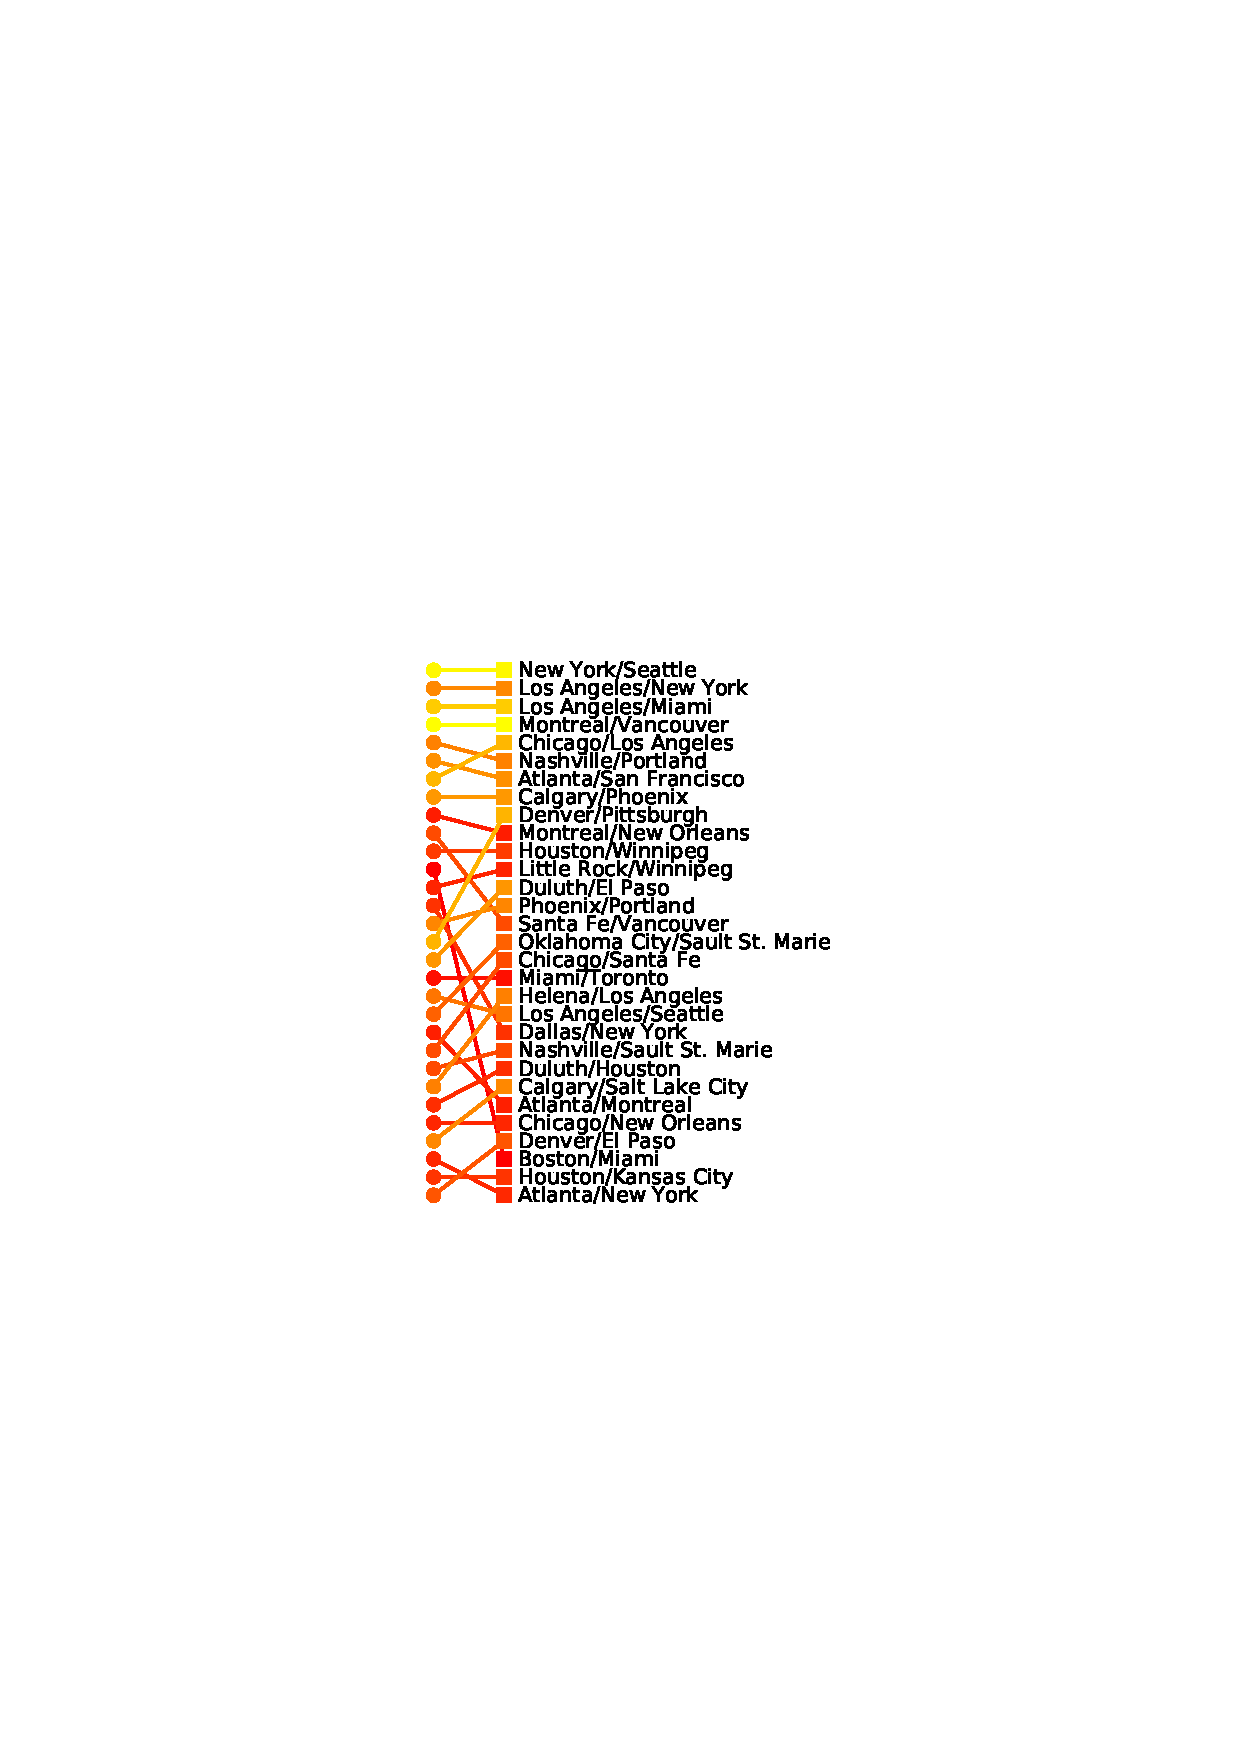
\includegraphics[scale=.25]{figures/rankings.png}
    \caption{Destination Tickets ordered by path length
    in the left column (circles) and by residual
    in the right column (squares). The color
    corresponds to the proportion of overall wins (scale
    from \cref{fig:resistance}).
    Lines indicate the change in rank between
    the two orderings.}
    \label{fig:rankings}
\end{figure}

